\section{Set-up}\label{sec:setup}
The study of QHE requires a two-dimensional or quasi two-dimensional system.
In this experiment, a quantum well is created by trapping electrons in a thin layer of HgTe between two layers of HgCdTe. Due to the smaller band gap of HgTe compared to HgCdTe, a quantum well is formed. 
At low temperatures, 
\begin{align}
    k_\text{B}T << E_1-E_0
\end{align}
all electrons occupy the lowest energy level in direction of the confinement. 
This creates a two-dimensional electron gas (2DEG).
The sample is designed in a common Hall bar geometry with $8$ contacts at the edges with an additional pair for the gate voltage (see fig.\,\ref{fig:HallBar}).
The gate voltage is set to $V_\text g = -0.25V$ unless otherwise specified.
\begin{figure}[h]
    \centering
    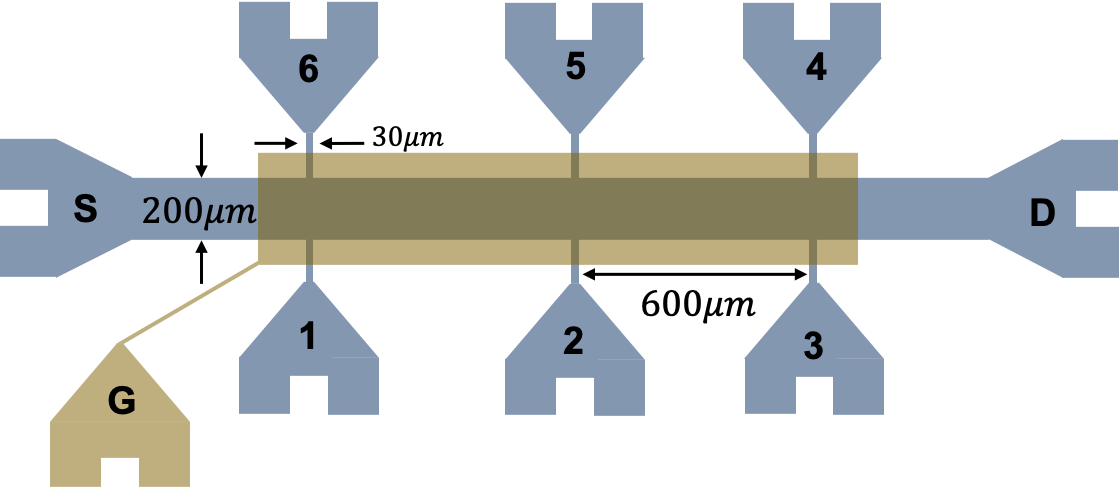
\includegraphics[width=0.45\textwidth]{../Images/HallBar.png}
    \caption{Schematic of the Hall Bar geometry. The contacts are labeled "S" 
    for source, "D" for drain, "G" for gate. Contacts $4$ and $6$ are used to 
    measure the longitudinal resistance and contacts $3$ and $4$ are used to measure 
    the transversal resistance.}
    \label{fig:HallBar}
\end{figure}
An AC voltage is applied between the source and drain to control the longitudinal current $I$ flowing through the sample. 
$I$ can be measured by the voltage drop $U_\text{I}$ across a known resistor 
$(R_\text{S}=4.982\pm0.0005)\,\text{k}\Omega$ connected in series with the source contact. 
$U_\text{I}$ is measured with a lock-in amplifier \emph{Stanford Research Systems SR510}. 
Contacts $3$ and $4$ are used to measure the Hall voltage $U_\text{Hall}$, which is measured with a second lock-in amplifier of the same type. 
Contacts $4$ and $6$ are used to measure the longitudinal voltage $U_\text{xx}$, which is measured with a third lock-in amplifier \emph{Stanford Research Systems SR530}.
All lock-in amplifiers use a phase-sensitive amplification approach by filtering the noise by multiplying the signal with a $13\,\text{Hz}$ reference signal. The data is then integrated over a period of $3\,\text{s}$ and measured with a sensitivity of $1\,\text{mV}$.
The gain accuracy is $1\%$.
The Hall bar sample has a width of $200\,\mu\text{m}$ and a length of $1200\,\mu\text{m}$, as shown in fig.\,\ref{fig:HallBar}.\\
To observe the Hall effect, a magnetic field $B$ is applied perpendicular to the plane of the sample.
The magnetic field is generated by a superconducting NbTi magnet cooled with liquid helium. 
$B$ can be precisely controlled by the current flowing through the magnet. 
$B$ is read out as voltage $U_\text{B}$ where $U_\text{B}=10\,\text{V}$ corresponds 
to $9\,\text{T}$.
The Hall bar is placed inside a variable temperature insert (VTI), which allows the sample to be cooled by evaporating liquid He at different pressures. 
Measurements are made at the temperatures $\csname tempFor4.2K\endcsname$, 
$\csname tempFor3K\endcsname$, $\csname tempFor2.1K\endcsname$, $\csname tempFor1.4K\endcsname$, 
which will be referred to as the target temperatures $4.2 \,\text K$, $3 \,\text K$, $2.1 \,\text K$, and $1.4 \,\text K$, respectively.
The temperature of the sample is measured by the voltage drop across an $Alan Bradley$ resistor $R_\text{AB}=100\,\Omega$ using a \emph{Keithley 160B} digital multimeter and a constant current of $10\,\mu\text{m}$.
Acting as a resistive thermometer, the carbon resistor is placed with the sample inside the VTI and is calibrated for the temperature range used.
The conversion from voltage to temperature is done with the calibration table \cite{ExperimentDescription}. \\
The temperatures could not be stabilized perfectly, so the average temperature between the beginning and the end of the measurement is being used.
While the magnetic field is turned on, the temperature could not be measured because the resistance depends on the magnetic field.
Since the resistor is not exactly positioned on the Hall bar and its error is not known, the temperature error is estimated to be $1\%$.
If half of the temperature drift is larger than this error, it is used as the error instead.


